% !TEX program = xelatex
% !BIB program = bibtex
\documentclass[a4paper, 12pt, oldfontcommands, final]{memoir}
\settrimmedsize{9.5in}{6.8in}{*}           % 9.5in X 6.8in
\settrims{79.136pt}{53.118pt}              % 
\settypeblocksize{7.8in}{5in}{*}           % 7.8in X 5.2in
\setlrmargins{*}{*}{1}                     % S=0.7in
\setulmargins{*}{*}{.7}                    % U=0.55in+0.3in for header
\trimXmarks
\checkandfixthelayout
\nonstopmode

\usepackage{bookstyle}

% set header
\makepagestyle{mystyle}% name
  \makeevenhead{mystyle}{\thepage}{}{\itshape কম্বিনেটরিকসে হাতেখড়ি}% Even page header
  \makeoddhead{mystyle}{\itshape\rightmark}{}{\thepage}% Odd page header
  \nouppercaseheads
  % Set page style to 'mystyle'
  \pagestyle{mystyle}

\title{কম্বিনেটরিকসে হাতেখড়ি}
\author{আদীব হাসান\\
জয়দীপ সাহা\\
আহমেদ জাওয়াদ চৌধুরী}

\begin{document}
\frontmatter
\thispagestyle{empty}
\maketitle
\vspace*{\fill}
\begin{center}
	\uccoff{\fontfamily{lmr}\selectfont ©} ২০১৯~~আদীব হাসান
	\pagebreak
\end{center}

\tableofcontents*

\mainmatter
% section counter resets with chapter counter
\counterwithin{section}{chapter}
% translate section counter to bangla
\renewcommand\thesection{\thechapter.\tobangla{section}}
% page counter in bangla
\renewcommand{\thepage}{\tobangla{page}}
% Since mainmatter resets \thefigure to \arabic
% translate it back to bangla
\renewcommand{\thefigure}{\thechapter.\tobangla{figure}}

% the chapters that are commented out are not actually in the repo.
% this is just to demonstrate how your project should look like.

% \include{chap/counting_basic}
% \include{chap/probability}
% !TEX root=../main.tex
\newcommand{\phpname}{পিজিয়নহোল প্রিন্সিপল}
\newcommand{\phpnamer}{পিজিয়নহোল প্রিন্সিপলের}
\chapter[পিজিয়নহোল প্রিন্সিপল (Pigeonhole Principle)]{পিজিয়নহোল প্রিন্সিপল}
\begin{chapquote}{Gary Lineker}
	Football is a simple game. Twenty-two men chase a ball for 90 minutes and at the end, the Germans always win.
\end{chapquote}
\vspace{-2em}
\section{সরল (Simple) \phpname{}}
\firstword{ম}{নে} করো, তোমার কাছে $(n+1)$-সংখ্যক পায়রা আছে, আর এদেরকে তুমি $n$-সংখ্যক খোপে রাখতে চাও। তাহলে, নিশ্চয়ই তোমাকে অন্তত একটি খোপে একাধিক পায়রা রাখতে হবে? এই সাদাসিধে ধারণাটিকে বলে \phpname{} বা সোজা বাংলায় পায়রার খোপ নীতি।
\begin{figure}[hbt]
\centering
\includegraphics[width=0.5\linewidth]{img/pigeonhole_principle/pigeonhole}
\caption{$(n+1)$-সংখ্যক পায়রা আর $n$-সংখ্যক খোপ।}
\end{figure}

তবে সাদাসিধে হলেও \phpname{} অত্যন্ত কাজের একটি জিনিস। কেননা ঠিক ঠিক গাণিতিক বস্তুকে পায়রা এবং খোপ হিসেবে চিন্তা করে এর সাহায্যে অনেক বাঘা বাঘা উপপাদ্য প্রমাণ করে ফেলা সম্ভব। \phpname{} ব্যবহার হয় এমন কিছু সমস্যা চলো তাহলে দেখি!

\begin{example}
	প্রমাণ করো সাত ভাই চম্পা ও পারুলের মধ্যে অন্তত দুইজনের জন্ম একই বারে!
\end{example}
\begin{solution}
	আট ভাইবোনকে পায়রা এবং সপ্তাহের সাত দিনকে খোপ ভাবো। তাহলে অন্তত দুজন ভাইবোন (পায়রা)-কে একই খোপে যেতে হবে, অর্থাৎ একই বারে জন্মাতে হবে।
\end{solution}
\begin{example}
	ময়মনসিংহ জিলা স্কুলে $2000$ জন ছাত্র পড়ে। প্রমাণ করো অন্তত দুইজন ছাত্রের জন্মদিন বছরের একই দিনে।
\end{example}
\begin{solution}
	ছাত্রদেরকে পায়রা এবং বছরের $365$ দিনকে খোপ ধরো। অবশ্যই একাধিক ছাত্রকে কোনো একটি খোপে যেতে হবে, অর্থাৎ একই দিনে জন্মাতে হবে।
\end{solution}
\begin{example}
	আমরা জানি যে-কোনো মানুষের মাথায় $3$ লক্ষের বেশি চুল থাকে না। এবার প্রমাণ করো ঢাকা শহরে অন্তত দুইজন মানুষের মাথায় সমান সংখ্যক চুল আছে!
\end{example}
\begin{solution}
	ঢাকা শহরের জনসংখ্যা $3$ লক্ষের চেয়ে অনেক বেশি। যদি চুলের সংখ্যাকে পায়রার খোপ আর মানুষের মাথাকে পায়রা হিসেবে চিন্তা করি, তবে \phpname{} অনুসারে একটি নির্দিষ্ট সংখ্যার চুল অবশ্যই একাধিক মানুষের মাথায় থাকবে।
\end{solution}
\begin{remark}
	ঢাকার সব টেকো লোকের মাথায় বাই ডেফিনিশন $0$টি চুল আছে। ওপরের সমস্যার একটি হাস্যকর সমাধান এটি হতে পারে। তবে যদি সব টেকো লোককে বাদ দিয়ে চুলের সংখ্যা গোণা হয়, তাও ওপরের সমাধান অনুযায়ী ঢাকার অন্তত দুইজন লোকের মাথায় সমান সংখ্যক চুল পাওয়া যাবে।
\end{remark}


\begin{example}
	প্রমাণ করো $(n+1)$-সংখ্যক পূর্ণসংখ্যার প্রতিটিকে $n$ দিয়ে ভাগ করা হলে অন্তত দুটি সংখ্যার ভাগশেষ অভিন্ন হবে।
\end{example}
\begin{solution}
	আমরা জানি, কোনো সংখ্যাকে $n$ দিয়ে ভাগ করলে $n$-সংখ্যক সংখ্যা 0, 1, 2, $\ldots$, $n-1$-এর মধ্যে যে-কোনো একটি ভাগশেষ হবে। এখন সম্ভাব্য ভাগশেষগুলোকে খোপ আর $(n+1)$-সংখ্যক সংখ্যাকে পায়রা ধরলে কমপক্ষে দুটি সংখ্যাকে অবশ্যই একই খোপে যেতে হবে। তাই এদেরকে $n$ দিয়ে ভাগ করলে ভাগশেষ সমান হবে।
\end{solution}

\begin{example}
	দেখাও যে প্রতিটি ধনাত্মক পূর্ণসংখ্যা $n$-এর এমন একটি ধনাত্মক গুণিতক আছে যা শুধুমাত্র $0$ এবং $5$ দিয়ে গঠিত।
\end{example}
\begin{solution}
	নিচের $(n+1)$-সংখ্যক সংখ্যার যে-কোনো দুটির পার্থক্য হবে শুধুমাত্র $0$ ও $5$ দিয়ে গঠিত কোনো সংখ্যা।
	\[5, \;55, \;555, \;\ldots,\;\underbrace{5\ldots5}_{(n+1)\text{ টি}}\]
	আবার, আগের উদাহরণ  অনুযায়ী, এই $(n+1)$-সংখ্যক সংখ্যার মধ্যে অন্তত দুটি সংখ্যা আছে যাদের $n$ দিয়ে ভাগ করলে অভিন্ন ভাগশেষ থাকবে। অতএব, এই দুটি সংখ্যার পার্থক্যই $n$-এর কাঙ্ক্ষিত একটি গুণিতক।
\end{solution}

\begin{example}
	একটি $1$ মিটার বাহুবিশিষ্ট সুষম ষড়ভুজের ভেতরে $7$টি বিন্দু নেওয়া হলো। প্রমাণ করো যে, এদের মধ্যে অন্তত দুটি বিন্দুর মধ্যবর্তী দূরত্ব $1$ মিটার থেকে বেশি নয়।
\end{example}

\begin{figure}[htb]
	\centering
	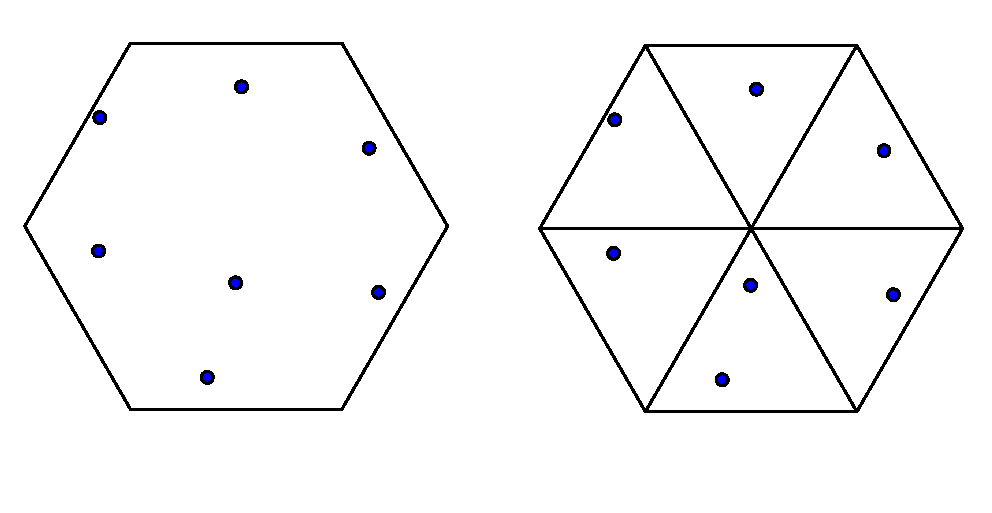
\includegraphics[width=0.6\textwidth]{img/pigeonhole_principle/points-in-hexagon}
	\caption{ষড়ভুজের ভেতর $7$টি বিন্দু।}\label{php-figure-points-in-hexagon}
\end{figure}

\begin{solution}
	\autoref{php-figure-points-in-hexagon}-এর মতো ষড়ভুজটিকে ছয়টি সমবাহু ত্রিভুজে বিভক্ত করো। এই ছয়টি ত্রিভুজকে খোপ আর সাতটি বিন্দুকে পায়রা ভাবলে, \phpname{} অনুসারে অন্তত একটি ত্রিভুজের ভেতরে একাধিক বিন্দু পড়বে। এখন প্রতিটি ত্রিভুজের বাহুর দৈর্ঘ্য যেহেতু $1$ মিটার, তাই সেই দুটি বিন্দুর মধ্যবর্তী দূরত্ব $1$ মিটারের চেয়ে বেশি হতে পারে না।
\end{solution}

\section{বর্ধিত \phpname}
মনে করো, তুমি $7$টি পায়রাকে $3$টি খোপে রাখতে চাও। অন্তত একটি খোপে নিশ্চয়ই তোমাকে $3$টি পায়রা রাখতে হবে, কেননা কোনো খোপে দুটির বেশি পায়রা না রাখলে $3$টি খোপে সর্বোচ্চ $3\times2=6$টি পায়রা রাখা যেতে পারে। তেমনিভাবে, যদি  $m$-সংখ্যক পায়রাকে $n$-সংখ্যক খোপে রাখা হয়, তবে একটি খোপে অন্তত $\left\lceil\frac{m}{n}\right\rceil$-সংখ্যক পায়রা থাকবে।\footnote{$\lceil\ \rceil$ বা সিলিং ফাংশন(পরিশিষ্ট দেখো)} এটি \phpnamer{} বর্ধিত রূপ।

\begin{example}
	তিনটি স্বাভাবিক সংখ্যার যোগফল $17$ হলে দেখাও যে অন্তত একটি পূর্ণসংখ্যা $5$-এর চেয়ে বড়ো।
\end{example}
\begin{solution}
	সংখ্যা তিনটিকে খোপ হিসেবে চিন্তা করো। $17$টি পায়রাকে $3$টি খোপে রাখতে গেলে একটি খোপে অবশ্যই $\left\lceil\frac{17}{3}\right\rceil>5$টি পায়রা রাখতে হবে।
\end{solution}

\begin{example}
	প্রমাণ করো যে $\{1,2,\ldots,100\}$ সেটটি থেকে $51$টি ভিন্ন সংখ্যা তুলতে হলে অবশ্যই দুটি ক্রমিক সংখ্যা তুলতে হবে।
\end{example}
\begin{solution}
	যেহেতু আমাদের প্রমাণ করতে হবে অন্তত দুটি সংখ্যা ক্রমিক, আমরা উলটোটি করার চেষ্টা করি। অর্থাৎ দুটি সংখ্যা ক্রমিক না নিয়ে ওপরের সেট থেকে $51$টি সংখ্যা নেওয়ার চেষ্টা করি। প্রথমেই যেটি মাথায় আসতে পারে-
	\[\{1, 3, 5, 7,\ldots, 99\}\]
	কিন্তু এভাবে সর্বোচ্চ $50$টি সংখ্যা তোলা যাবে। পরের সংখ্যাটি অবশ্যই কোনো না কোনো সংখ্যার সঙ্গে ক্রমিক হবে। আমাদের প্রমাণ কিন্তু শেষ হয়ে যায়নি। কেননা আমরা এই ধারাটিও নিতে পারতাম-
	\[\{2, 4, 6, 8, \ldots, 100\}\]
	এবং একই যুক্তিতে সেটিও গ্রহণযোগ্য হতো না। আমরা ইচ্ছেমতো সংখ্যা তোলার চেষ্টাও করতে পারি। কিন্তু আমরা যতই ক্রমিক সংখ্যা না রেখে সংখ্যা নেবার চেষ্টা করি, আমরা দেখতে পাব যে $50$টির বেশি সংখ্যা কখনও নেওয়া যাচ্ছে না। এমন পরিস্থিতিতে পড়লেই আমরা \phpname{} ব্যবহার করে থাকি।

	এই সমস্যার সমাধানের জন্য খোপ হিসেবে নেব নিচের $50$টি ক্রমিক সংখ্যার ক্রমজোড়কে।
	\[(1, 2),\;(3, 4),\;(5, 6),\;\ldots,\;(99, 100)\]
	এবার আমাদের তোলা প্রতিটি সংখ্যাকে তার নিজের খোপে রাখব। যেমন, আমাদের $51$টি সংখ্যার মধ্যে 5 থাকলে তাকে আমরা রাখব $(5,6)$-তে। যেহেতু পায়রা $51$টি ও খোপ $50$টি, তাই অন্তত একটি খোপে আমাদেরকে দুটি পায়রা রাখতেই হবে। অর্থাৎ, সেই ক্রমজোড়ের দুটি ক্রমিক সংখ্যাই আমাদের তোলা $51$টি সংখ্যার মধ্যে থাকবে।
\end{solution}

\begin{example}(আইএমও ১৯৭২/১)
	তোমাকে $100$-এর চেয়ে ছোটো $10$টি  ধনাত্মক পূর্ণসংখ্যার একটি সেট দেওয়া আছে। প্রমাণ করো যে, এই সেটের এমন দুটি অশূন্য (non-empty), ডিসজয়েন্ট সাবসেট আছে যাদের উপাদানগুলোর যোগফল সমান।
\end{example}
\begin{solution}
	আইএমওর সমস্যা বলে একে ভয় পাওয়ার কিছু নেই। এটিও আমরা \phpnamer{} সাহায্যে চমৎকারভাবে ঘায়েল করতে পারি।

	\phpname{} প্রয়োগ করতে হলে আমাদের পায়রা আর খোপ লাগবে। তাই, চলো এখানে আমরা পায়রা এবং খোপ খুঁজি। প্রশ্নে দুটি ডিসজয়েন্ট সেটের উপাদানগুলোর যোগফল \textit{সমান} দেখাতে বলা হয়েছে। তাই আমরা প্রদত্ত সেটটির সব সাবসেটকে পায়রা, এবং এদের উপাদানগুলোর সম্ভাব্য যোগফলগুলোকে খোপ ধরব।

	প্রদত্ত সেটে যেহেতু $10$টি সংখ্যা আছে, তাই এর সাবসেট আছে $2^{10}=1024$টি। আবার, প্রদত্ত সেটের উপাদানগুলো যেহেতু $100$-এর চেয়ে ছোটো, তাই এর সবচেয়ে বড়ো সম্ভাব্য সাবসেটটি হতে পারে $\{99,\; 98,\; 97,\; 96,\; 95,\; 94,\; 93,\; 92,\; 91,\; 90\}$, যার উপাদানগুলোর যোগফল $945$. আর এর সবচেয়ে ছোটো সাবসেটটি হলো ফাঁকা সেট, যার যোগফল $0$. তাই, প্রদত্ত সেটের যে-কোনো সাবসেটের উপাদানগুলোর যোগফল হবে $0$ থেকে $945$-এর মধ্যে কোনো একটি পূর্ণসংখ্যা। সুতরাং সম্ভাব্য যোগফল অর্থাৎ খোপ আছে $945+1=946$টি।

	যেহেতু, $1024>946$, তাই \phpname{} অনুসারে প্রদত্ত সেটের এমন অন্তত দুটি সাবসেট অবশ্যই পাওয়া যাবে যাদের উপাদানগুলোর যোগফল সমান। কিন্তু সেই সাবসেট দুটি ডিসজয়েন্ট নাও হতে পারে! এদেরকে ডিসজয়েন্ট বানানোর জন্য আমরা এদের কমন উপাদানগুলো দুটি সাবসেট থেকে বাদ দেব। এর ফলে দুটি সাবসেটের উপাদানগুলোর যোগফল কমলেও সেগুলো পরস্পর সমানই থাকবে। লক্ষ্য করো যে, কমন উপাদান বাদ দেওয়ার পর কোনো সাবসেট ফাঁকা হয়ে যেতে পারে না। কারণ যদি দুটি সাবসেট ফাঁকা হয়ে যায়, তাহলে প্রথমেই সাবসেট দুটো অভিন্ন ছিল, যা অসম্ভব। আবার, কেবল একটি সাবসেট ফাঁকা হলে ঐ সাবসেটের উপাদানগুলোর যোগফল শূন্য, যেখানে অপর সাবসেটের উপাদানগুলোর যোগফল ধনাত্মক। তাই তারা সমান হতে পারে না। অতএব সেটিও সম্ভব নয়।

	তাহলে, আমরা প্রদত্ত সেটের দুটি ডিসজয়েন্ট সাবসেট পেয়ে গেলাম যাদের যোগফল সমান।
\end{solution}

\begin{example}(বিডিএমও ২০১৪, জুনিয়র ১০)
	ঐন্দ্রির কাছে $100$টি চকলেট ছিল। সে $58$ দিনে সবগুলো চকলেট খেয়ে শেষ করে। সে প্রতিদিন কমপক্ষে একটি করে চকলেট খেয়েছে। প্রমাণ করো যে, ঐন্দ্রি পর পর কয়েক দিনে ঠিক $15$টি চকলেট খেয়েছে।
\end{example}
\begin{solution}
	ধরা যাক, ঐন্দ্রি শুরু থেকে $i$-তম দিন পর্যন্ত মোট $a_i$-সংখ্যক চকলেট খেয়েছে। সে প্রতিদিনই কমপক্ষে একটি চকলেট খেয়েছে। সুতরাং,
	\begin{align*}
		0<a_1 < a_2 < \cdots < a_{58}&=100 \\
		\implies a_1+15 < a_2+15<\cdots < a_{58}+15&=115
	\end{align*}
	এখন $a_1,\ a_2,\ \ldots,\ a_{58},\ (a_1+15),\ (a_2+15),\ \ldots,\ (a_{58}+15)$ পর্যন্ত $58+58=116$টি সংখ্যাকে পায়রা এবং এদের মান, অর্থাৎ $1$ থেকে $115$ পর্যন্ত সংখ্যাকে খোপ ধরো। তাহলে, \phpname{} অনুযায়ী এদের মধ্যে অন্তত দুটি সংখ্যার মান সমান। অর্থাৎ, এমন দুটি দিন $m$ এবং $n$ আছে যাতে করে $a_m = a_n+15$ হয়। $n$-তম এবং $m$-তম দিনের মধ্যে ঐন্দ্রি সব মিলিয়ে ঠিক ঠিক $15$টি চকলেট খেয়েছে।
\end{solution}

বেশিরভাগ সমস্যায় মূল ধাপ থাকে পায়রা এবং খোপ চিহ্নিত করা। আবার, কঠিন সমস্যাগুলোতে \phpname{} একটি মধ্যবর্তী ধাপ হিসেবে ব্যবহার করা হয়, তা সম্পূর্ণ সমাধান দেয় না। যেমন-- পরবর্তী সমস্যাটি দেখো।

\begin{example}
	জাহিন একটি বোর্ডে $70$-এর চেয়ে ছোটো $20$টি ভিন্ন ভিন্ন ধনাত্মক পূর্ণসংখ্যা নিলো এবং এদের সবরকমের জোড়ার পার্থক্য অন্য একটি বোর্ডে লিখল। প্রমাণ করো, দ্বিতীয় বোর্ডে $4$টি সংখ্যা আছে যেগুলো পরস্পর সমান।
\end{example}

\begin{solution}
	কাউন্টিং-এর জ্ঞান কাজে লাগিয়ে আমরা বলতে পারি যে দ্বিতীয় বোর্ডে $\binom{20}{2}=190$টি সংখ্যা আছে। এই সংখ্যাগুলো হবে আমাদের পায়রা।

	প্রথম বোর্ডে সবচেয়ে বড়ো সংখ্যা হতে পারে $69$, এবং সবচেয়ে ছোটো সংখ্যা হতে পারে $1$. তাই দ্বিতীয় বোর্ডে কোনো সংখ্যার সম্ভাব্য সর্বোচ্চ মান $69-1=68$ এবং সম্ভাব্য সব মান হচ্ছে $1$ থেকে $68$ পর্যন্ত $68$টি ভিন্ন ভিন্ন সংখ্যা। এদের আমরা খোপ ধরলে \phpname{} অনুসারে দ্বিতীয় বোর্ডে অন্তত $\left\lceil\frac{190}{68}\right\rceil=3$টি সংখ্যা একই হবে।

	কিন্তু এ কী! আমদের দেখাতে হবে দ্বিতীয় বোর্ডে অন্তত $4$টি সংখ্যা একই হবে। এবার কী করা যায়?

	আমরা আরেকটু চেষ্টা করি। চলো, প্রথমে সংখ্যাগুলোকে ছোটো থেকে বড়ো ক্রমে সাজাই এবং ধরি, সংখ্যাগুলো $a_1, a_2, a_3, \ldots, a_{20}$. তাহলে দ্বিতীয় বোর্ডের সংখ্যাগুলো হবে $a_i-a_j$, যেখানে $i>j$. ধরো $(a_2-a_1)$, $(a_3-a_2)$, $(a_4-a_3),\ \ldots,\ (a_{20}-a_{19})$-এর কোনোটিই দ্বিতীয় বোর্ডে $3$ বারের বেশি নেই। তাহলে $a_{20}-a_{1}$-এর সর্বনিম্ন মান হতে পারে,
	\begin{align*}
		a_{20}-a_1 &= (a_{20}-a_{19})+ (a_{19}-a_{18})+\ldots+(a_2-a_1)\\
				  &\ge 3\times 1+3\times 2+\ldots +3\times 6 +7\\
				  &=70
	\end{align*}
	কিন্তু $(a_{20}-a_{1})$ সংখ্যাটি দ্বিতীয় বোর্ডে আছে বিধায় এটি $68$-এর বেশি হতে পারে না। তাই আমরা যা ধরে নিয়েছিলাম সেটি ভুল। তাই একটি না একটি $(a_{i+1}-a_i)$ কমপক্ষে $4$ বার দ্বিতীয় বোর্ডে আছে। তাই দ্বিতীয় বোর্ডে এই সংখ্যাটি অন্তত $4$ বার লেখা হয়েছে।
\end{solution}

আমাদের কিছু পরিচিত ফাংশন রয়েছে, যেগুলো নিয়ে ধারণা থাকলে কিছু সমস্যা সমাধানে সুবিধা হতে পারে। যেমন ধরো $\tan$ ফাংশন। এর বিয়োগের সূত্রটি হচ্ছে,
\[\tan (A-B)=\frac{\tan A - \tan B}{1+\tan A \tan B}\]
এটি জানা থাকলে পরবর্তী সমস্যাটির একটি সুন্দর সমাধান বের করা সম্ভব।
\begin{example}
	দেখাও যে, যে-কোনো $5$টি বাস্তব সংখ্যার মধ্যে এমন দুটি সংখ্যা $a$ আর $b$ পাওয়া যাবে, যারা নিচের অসমতাটি মেনে চলে
	\[0<\dfrac{a-b}{1+ab}<1\]
\end{example}
\begin{solution}
	এই সমস্যার শর্তটির সঙ্গে $\tan$-এর বিয়োগের সুত্রের কি মিল পাচ্ছ? ব্যাপারটি এমন যেন, $a$ এবং $b$ দুটি $\tan$-এর মান। তাই আমরা পাঁচটি সংখ্যার $\tan ^{-1}$ নেব, এবং ধরব মানগুলো হচ্ছে $x_1,\ x_2,\ x_3,\ x_4$ এবং $x_5$. তাহলে,
	\[-\frac{\pi}{2}<x_1,\;x_2,\; x_3,\; x_4,\; x_5<\frac{\pi}{2}\]
	এখন $(-\frac\pi 2,\frac\pi 2)$ ব্যবধিকে আমরা $4$টি সমান ভাগে ভাগ করি। প্রতিটি ভাগের দৈর্ঘ্য তাহলে (প্রায়) $\frac \pi 4$. \phpname{} অনুযায়ী কোনো একটি ভাগে দুটি সংখ্যা পড়বে। এদের পার্থক্য নিশ্চয়ই তাহলে $\frac\pi 4$ থেকে ছোটো। মনে করি, এই সংখ্যা দুটি $p$ ও $q$. তাহলে, $a=\tan p$ ও $b=\tan q$. এবং আমাদের প্রাপ্ত শর্তানুসারে,
	\[0 < \tan(p-q) < \tan \left(\frac{\pi}{4}\right)\]
	$\tan$-এর বিয়োগের সূত্র প্রয়োগ করে লেখা যায়,
	\[0 < \frac{\tan p - \tan q}{1+\tan p\tan q} < 1\]
	যেটি সরল করলে হয়,
	\[0 < \frac{a-b}{1+ab} < 1\]
\end{solution}

\begin{example}[label=php-six-facebook-users-example]
	প্রমাণ করো তোমার ক্লাসের $6$ জন ফেসবুক ব্যবহারকারীর মধ্যে হয় এমন $3$ জন আছে যারা প্রত্যেকে প্রত্যেকের ফ্রেন্ড, নাহয় এমন $3$ জন আছে যারা কেউ কারও ফ্রেন্ড নয়।
\end{example}
\begin{figure}[hbt]
	\centering
	\begin{tabular}{cc}
	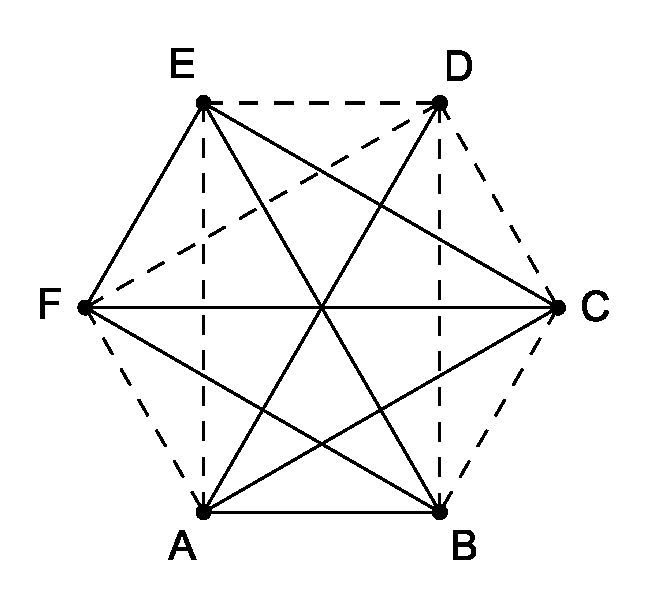
\includegraphics[width=0.35\textwidth]{img/pigeonhole_principle/six-facebook-users-full}
	&
	\includegraphics[width=0.35\textwidth]{img/pigeonhole_principle/six-facebook-users-partial}\\
	(ক) পূর্ণাঙ্গ ফ্রেন্ডশিপ ম্যাপ। & (খ) প্রমাণের জন্য দরকারী অংশ।
	\end{tabular}
	\caption{ছয় ফেসবুক ব্যবহারকারীর ফ্রেন্ডশিপ ম্যাপ।}
	\label{php-six-facebook-users}
\end{figure}
\begin{solution}
	মনে করো, $A$, $B$, $C$, $D$, $E$, এবং $F$ হলো তোমার ক্লাসের $6$ জন ফেসবুক ব্যবহারকারী। এদেরকে শীর্ষবিন্দু ধরে একটি সুষম ষড়ভুজ আঁকো। দুজন ফেসবুক ব্যবহারকারী পরস্পরের ফ্রেন্ড হলে তাদেরকে একটি সলিড রেখাংশ (---), এবং ফ্রেন্ড না হলে তাদেরকে একটি ড্যাশ রেখাংশ (-\,-) দিয়ে সংযুক্ত করে দাও। এই ছবিটিকে আমরা বলব ফ্রেন্ডশিপ ম্যাপ। উদাহরণস্বরূপ, \autoref{php-six-facebook-users}(ক)-তে ছয় ফেসবুক ব্যবহারকারীর মধ্যকার ফ্রেন্ডশিপের একটি সম্ভাব্য ম্যাপ আঁকা হয়েছে। তবে তোমার ম্যাপটি ঠিক এরকমই হতে হবে এমন কোনো কথা নেই।

	তিন জন ফেসবুক ব্যবহারকারী প্রত্যেকে প্রত্যেকের ফ্রেন্ড হওয়ার অর্থ এই ফ্রেন্ডশিপ ম্যাপে একটি সলিড রেখাংশের ত্রিভুজ থাকা। তেমনিভাবে, তিন জন কেউ কারও ফ্রেন্ড না হওয়ার মানে এখানে একটি ড্যাশ রেখাংশের ত্রিভুজ থাকা। সুতরাং, আমাদেরকে প্রমাণ করতে হবে যে, ছয়জন মানুষের ফ্রেন্ডশিপ ম্যাপটি যেভাবেই গঠিত হোক না কেনো, এতে একই রকমের রেখাংশ দিয়ে তৈরি অন্তত একটি ত্রিভুজ থাকবে।

	এই স্টেটমেন্টটি প্রমাণ করার জন্য আমরা \autoref{php-six-facebook-users}(ক) থেকে কিছু রেখাংশ মুছে দিয়ে একটি সরল \autoref{php-six-facebook-users}(খ) আঁকব। এখানে $A$-র সঙ্গে অন্য পাঁচ জন পাঁচটি রেখাংশ দিয়ে যুক্ত আছে(ছবি \autoref{php-six-facebook-users}(খ))। এই পাঁচটি রেখাংশকে পায়রা এবং রেখাংশের ধরণকে খোপ ধরলে \phpname{} অনুযায়ী অন্তত তিনটি রেখাংশ একই রকম হতে হবে। ধরা যাক, তিনটি রেখাংশ $AB, AC$ এবং $AD$ হচ্ছে সলিড (---)। (অন্তত তিনটি রেখাংশ ড্যাশ (-\,-) হলেও অনুরূপভাবে প্রমাণ করা যাবে।) এখন $BC$ রেখাংশ যদি সলিড হয়, তবে $ABC$ একটি সলিড রেখার ত্রিভুজ হয়ে যাবে। সেক্ষেত্রে আমাদের প্রমাণ শেষ। আর তা যদি না হয়, তবে $BC$ একটি ড্যাশ রেখাংশ। একই যুক্তিতে $CD$ এবং $BD$-ও ড্যাশ রেখাংশ হবে। কিন্তু সেক্ষেত্রে $BCD$ একটি ড্যাশ রেখাংশের ত্রিভুজ হয়ে যায়। অতএব ফ্রেন্ডশিপ ম্যাপে সবসময়ই একটি একই ধরণের রেখাংশ দিয়ে তৈরি ত্রিভুজ পাওয়া যাবে। সুতরাং, যে-কোনো $6$ জন ফেসবুক ব্যবহারকারীর মধ্যে হয় এমন $3$ আছে যারা প্রত্যেকে প্রত্যেকের ফ্রেন্ড, নাহয় এমন $3$ জন আছে যারা কেউ কারও ফ্রেন্ড নয়।
\end{solution}
\begin{remark}
	এই সমস্যাটির জেনারেলাইজেশন হচ্ছে রামসে সংখ্যা (Ramsey Numbers)। প্রকৃতপক্ষে আমরা এখানে প্রমাণ করেছি যে $R(3,3)\leq 6$. গ্রাফ থিওরি অধ্যায়ে রামসে সংখ্যা নিয়ে বিস্তারিত আলোচনা পাবে।
\end{remark}

\begin{diybox}
	নিচের ঘটনাগুলো \phpname{} দিয়ে ব্যাখ্যা করতে পারবে কি?
	\begin{noindlist}
		\item যে-কোনো $13$ জন লোকের মধ্যে অন্তত $2$ জনের একই মাসে জন্ম হয়েছে।
		\item $6$ বিষয়ের কোনো পরীক্ষায় যদি কেউ $486$ পায়, তবে সে কমপক্ষে একটি পরীক্ষায় $81$ বা তার বেশি পেয়েছে।
		\item কোনো ওয়ানডে ম্যাচ এ যদি কোনো দল $250$ রান করে, তবে কমপক্ষে একটি ওভারে $5$ বা তার বেশি রান হয়েছে।
		\item প্রমাণ করো যে-কোনো বিয়েবাড়িতে এমন দুজন লোক অবশ্যই পাওয়া যাবে যারা সমান সংখ্যক লোকের সঙ্গে করমর্দন করেছে।
	\end{noindlist}
\end{diybox}

\section{\texorpdfstring{অসীম \phpname}{অসীম পিজিয়নহোল প্রিন্সিপল}}
যদি তোমার কাছে অসীম সংখ্যক পায়রা থাকে, আর তুমি তাদেরকে সসীম সংখ্যক খোপে রাখতে চাও, তবে অন্তত একটি খোপে অবশ্যই অসীম সংখ্যক পায়রা রাখতে হবে। \phpnamer{} এই রূপটি ব্যবহার করে অনেক সময় বেশ ট্রিকি সমস্যার সুন্দর সমাধান পাওয়া যায়। পরবর্তী উদাহরণটি দেখো।

\begin{example}
	রাজকুমারকে এক রাক্ষস \autoref{php-mayapuri}-এর মতো একটি $8\times8$ মায়াপুরীতে আটকে রেখেছে। মায়াপুরীর চারদিকে উঁচু দেয়াল রয়েছে, এবং এটি থেকে বেরোবার একমাত্র দরজাটি হচ্ছে উত্তর-পূর্ব কোণার ঘরটির পাশে। প্রতিটি ঘরের মেঝেতে একটি করে জাদুর তিরচিহ্ন আঁকা রয়েছে যা উত্তর, দক্ষিণ, পূর্ব, বা পশ্চিমে মুখ করে আছে। কোনো ঘরের তিরচিহ্ন যেদিকে মুখ করে থাকে, সেই ঘর থেকে শুধুমাত্র সেই দিকে পার্শ্ববর্তী ঘরে যাওয়া যায়। যদি কোনো ঘরের তিরচিহ্ন দেয়ালের দিকে মুখ করে থাকে, তবে অবশ্য সেখান থেকে অন্য কোনো ঘরে যাওয়া যায় না। রাজকুমার মায়াপুরীর যে ঘরে পা দেয়, সেই ঘরের তিরচিহ্নটি ঘড়ির কাঁটার দিকে $90^\circ$ ঘুরতে থাকে যতক্ষণ না সেটি কোনো ঘরের দিকে অথবা দরজাের দিকে মুখ করে। রাজকুমার মায়াপুরীর \textbf{যে-কোনো} একটি ঘর থেকে যদি তিরচিহ্ন অনুসরণ করে হাঁটতে থাকে, তবে কি সে মায়াপুরী থেকে বের হতে পারবে?
\end{example}
\begin{figure}[h]
\centering
\bgroup
\def\arraystretch{1.6}
\begin{tabular}{||c|c|c|c|c|c|c|c||}
\hhline{|t:========:t|}
$\uparrow$& $\rightarrow$ & $\rightarrow$&$\uparrow$& $\leftarrow$& $\downarrow$&$\downarrow$ & \multicolumn{1}{c}{$\uparrow$} \\
\hhline{||--------||}
$\downarrow$  & $\rightarrow$ & $\uparrow$    & $\uparrow$    & $\downarrow$  & $\downarrow$  & $\rightarrow$ & $\leftarrow$\\
\hhline{||--------||}
$\rightarrow$ & $\downarrow$  & $\leftarrow$  & $\rightarrow$ & $\downarrow$  & $\leftarrow$  & $\uparrow$    & $\downarrow$ \\
\hhline{||--------||}
$\leftarrow$  & $\rightarrow$ & $\leftarrow$  & $\downarrow$  & $\leftarrow$  & $\downarrow$  & $\rightarrow$ & $\leftarrow$ \\
\hhline{||--------||}
$\rightarrow$ & $\downarrow$  & $\uparrow$    & $\leftarrow$  & $\downarrow$  & $\uparrow$    & $\downarrow$  & $\uparrow$ \\
\hhline{||--------||}
$\downarrow$  & $\downarrow$  & $\leftarrow$  & $\uparrow$    & $\downarrow$  & $\rightarrow$ & $\downarrow$  & $\leftarrow$ \\
\hhline{||--------||}
$\downarrow$  & $\rightarrow$ & $\uparrow$    & $\leftarrow$  & $\rightarrow$ & $\rightarrow$ & $\leftarrow$  & $\downarrow$  \\
\hhline{||--------||}
$\rightarrow$ & $\uparrow$    & $\leftarrow$  & $\uparrow$    & $\downarrow$  & $\leftarrow$  & $\uparrow$    & $\rightarrow$\\
\hhline{|b:========:b|}
\end{tabular}
\egroup
\caption{মায়াপুরী ও দরজার অবস্থান।}
\label{php-mayapuri}
\end{figure}
\begin{solution}
	তুমি ভাবতে পারো যদি রাজকুমার উত্তর-পূর্ব কোণের ঘরটি থেকে হাঁটা শুরু করে, তাহলে প্রথমবারই ঘরের তিরচিহ্নটি দরজার দিকে মুখ করবে, এবং সে বের হয়ে যেতে পারবে। অতএব,কাজ শেষ। কিন্তু আসলেই কি শেষ? খেয়াল করে দেখো প্রশ্নে মোটা অক্ষরে বলা হয়েছিল রাজকুমার যে-কোনো ঘর থেকে চলা শুরু করতে পারে। সব বারই কি সে মায়াপুরী থেকে বের হয়ে যেতে পারবে? এর উত্তরটাও হচ্ছে, হ্যাঁ, পারবে। (কি মজা!)

	এটি প্রমাণ করার জন্য আগে আমাদের উলটোটি ধরে নিতে হবে। অর্থাৎ, মনে করো রাজকুমার কখনও মায়াপুরী থেকে বের হতে পারবে না। সে যেহেতু হাঁটা থামাচ্ছে না, সুতরাং সে অবশ্যই অসীম সময় ধরে একটির পর একটি ঘরে যেতে থাকবে। যেহেতু ঘরের সংখ্যা (খোপ) সসীম, অতএব, \phpname{} অনুসারে রাজকুমারকে অন্তত একটি ঘরে অবশ্যই অসীম সংখ্যকবার যেতে হবে। এখন খেয়াল করো, প্রতিবার রাজকুমার যখন এই ঘরটিতে পা দিচ্ছে, এই ঘরের তিরচিহ্নটি ঘড়ির কাঁটার দিকে $90^\circ$ ঘুরে যাচ্ছে। ফলে, এই ঘরের চারপাশে লাগোয়া চারটি ঘরেও রাজকুমার অসীম সংখ্যকবার যাবে। একই যুক্তিতে সে এই চারটি ঘরের চারপাশের ঘরগুলোতেও অসীম সংখ্যকবার যাবে। এই যুক্তি ধরে এগোতে থাকলে আমরা আসলে বুঝতে পারব যে মায়াপুরীর প্রতিটা ঘরেই রাজকুমার অসীম সংখ্যকবার যাবে। সুতরাং উত্তর-পূর্ব কোণার ঘরটিতেও সে অসীম সংখ্যকবার যাবে, এবং যখনই ঘরের তিরচিহ্ন দরজার দিকে মুখ করবে, সে বেরিয়ে আসবে।
\end{solution}

\section{এরডশ-সেকেরেশ (Erdös-Szekeres) উপপাদ্য}
মনে করো, আমাদের কাছে বাস্তব সংখ্যার একটি বড়োসড়ো ধারা আছে--
\[-2.5,\;0,\;5.1,\;4.3,\;0.11,\;0.9,\;-0.87,\;1.82,\;-3.2,\;1.85,\;-6.4,\;12,\;2.75\]
গণিত এবং প্রোগ্রামিং-এ মাঝেমধ্যেই আমাদের জানার প্রয়োজন পড়ে যে এমন ধারায় কত বড়ো ক্রমবর্ধমান (strictly increasing) বা ক্রমহ্রাসমান (strictly decreasing) উপধারা (subsequence) লুকিয়ে আছে। উদাহরণস্বরূপ, ওপরের ধারাটির একটি ক্রমবর্ধমান উপধারা হতে পারে--
\[-2.5,\ 0,\ 0.11,\ 0.9,\ 1.82,\ 1.85,\ 2.75\]
এবং ক্রমহ্রাসমান উপধারা হতে পারে
\[5.1,\ 4.3,\ 0.9,\ -0.87,\ -3.2,\ -6.4\]
প্রথম উপধারাটির দৈর্ঘ্য হচ্ছে $7$, ও দ্বিতীয়টির $6$. কিন্তু কোনো ধারা কত বড়ো হলে নিশ্চিতভাবে বলা যাবে যে তার একটি $7$ দৈর্ঘ্যের ক্রমবর্ধমান উপধারা, কিংবা $6$ দৈর্ঘ্যের ক্রমহ্রাসমান উপধারা থাকবে? এই প্রশ্নটির একটি চমৎকার উত্তর দেয় এরডশ-সেকেরেশ উপপাদ্য।

\begin{theorem}[এরডশ-সেকেরেশ, ১৯৩৫]
	যদি $m$ এবং $n$ দুটি ধনাত্মক পূর্ণসংখা হয়, এবং ভিন্ন ভিন্ন বাস্তব সংখ্যা দিয়ে গঠিত ধারায় অন্তত $(mn+1)$-সংখ্যক পদ থাকে, তবে এই ধারার $(m+1)$ দৈর্ঘ্যের একটি \textbf{ক্রমবর্ধমান} উপধারা, অথবা $(n+1)$ দৈর্ঘ্যের একটি \textbf{ক্রমহ্রাসমান} উপধারা থাকবে।
\end{theorem}
\begin{proof}
	মনে করো, ধারাটি \[c_1,\ c_2,\ c_3,\ \ldots,\ c_{mn+1}\]
	$c_1$ থেকে $c_i$-এর মধ্যে দীর্ঘতম ক্রমবর্ধমান উপধারার দৈর্ঘ্যকে $a_i$ এবং দীর্ঘতম ক্রমহ্রাসমান উপধারার দৈর্ঘ্যকে $b_i$ ধরো। যদি এই ধারার উপপাদ্যে বলা দৈর্ঘ্যের কোনো ক্রমবর্ধমান বা ক্রমহ্রাসমান উপধারা না থাকে, তবে নিশ্চয়ই এর সব ক্রমবর্ধমান উপধারার দৈর্ঘ্য হবে $m$ বা তার চেয়ে কম, এবং সব ক্রমহ্রাসমান ধারার দৈর্ঘ্য হবে $n$ বা তার চেয়ে কম। সুতরাং $(a_i,b_i)$ ক্রমজোড়টির সম্ভাব্য ভিন্ন ভিন্ন মান হতে পারে সর্বোচ্চ $m\times n=mn$-সংখ্যক। কিন্তু প্রদত্ত ধারায় পদ আছে $mn+1$-সংখ্যক। অতএব, \phpname{} অনুযায়ী প্রদত্ত ধারায় এমন দুটি পদ $c_j$ এবং $c_k$, $(j<k)$ আছে, যাদের জন্য $(a_j,b_j)= (a_k,b_k)$.

	লক্ষ্য করো যে $c_j$ এবং $c_k$ দুটি ভিন্ন ভিন্ন সংখ্যা। যদি $c_j < c_k$ হয়, তবে $c_k$-কে $a_j$ দৈর্ঘ্যের ক্রমবর্ধমান উপধারাটির সঙ্গে সংযুক্ত করে $c_1$ থেকে $c_k$-এর মধ্যে একটি $a_j+1$ দৈর্ঘ্যের ক্রমবর্ধমান উপধারা পাওয়া যাবে। অতএব $a_k\ge a_j+1>a_j$. আবার $c_k<c_j$ হলে, $c_k$-কে $b_j$ দৈর্ঘ্যের ক্রমহ্রাসমান উপধারাটির সঙ্গে সংসুক্ত করে $c_1$ থেকে $c_k$-র মধ্যে একটি $b_j+1$ দৈর্ঘ্যের ক্রমহ্রাসমান উপধারা পাওয়া যাবে। তাই, $b_k\ge b_j+1>b_j$. সুতরাং উভয়ক্ষেত্রেই আমরা পাচ্ছি যে একইসঙ্গে $a_j=a_k$ এবং $b_j=b_k$ হতে পারে না। তাই $(a_j,b_j)\neq (a_k,b_k)$.

	যেহেতু আমরা দুভাবে এগিয়ে দুরকম সিদ্ধান্তে পৌঁছুচ্ছি, এর অর্থ হচ্ছে আমরা প্রথমে যা ধরে নিয়েছিলাম সেটি ভুল। অর্থাৎ, প্রদত্ত ধারার অবশ্যই একটি $(m+1)$ দৈর্ঘ্যের ক্রমবর্ধমান উপধারা, অথবা $(n+1)$ দৈর্ঘ্যের ক্রমহ্রাসমান উপধারা থাকবে।
\end{proof}
এবার আমরা পিজিয়নহোল প্রিন্সিপলের একটি অত্যন্ত গুরুত্বপূর্ণ প্রয়োগ দেখব।

\section{ফাইনাইট অটোমাটা (Finite Automata)}
অনেক আগে যখন সবার হাতে-পকেটে কম্পিউটার ছিল না, তখন পৃথিবীর সবচেয়ে বুদ্ধিমান মানুষগুলো ভাবতো যদি কিছু বিশেষ বিশেষ হিসেব দ্রুত করতে পারে এমন একটি যন্ত্র কল্পনাতে বানানো যায়, তবে সেটি কোন কোন সমস্যা সমাধান করতে পারবে। বলাবাহুল্য বিভিন্ন মানুষের মাথায় এরকম নানা ধরণের কাল্পনিক গণনাযন্ত্রের আইডিয়া এসেছিল। ভিন্ন ভিন্ন বৈশিষ্ট্যসম্পন্ন সেসব কাল্পনিক যন্ত্রগুলোকে ডাকা হতো কম্পিউটেশন মডেল। তেমন একটি মডেলের নাম ফাইনাইট অটোমেটন (Automaton) বা বহুবচনে ফাইনাইট অটোমাটা। এটা পুরোপুরি কাল্পনিক একটি যন্ত্র। তবে আধুনিক ইলেক্ট্রনিক সার্কিট দিয়ে এটি সিমুলেট করা যায়। 

\begin{figure}[hbt]
	\centering
	\includegraphics[height=6cm]{img/pigeonhole_principle/101}
	\caption{একটি ফাইনাইট অটোমেটন।}
	\label{php-automata1}
\end{figure}

একটি ফাইনাইট অটোমেটনে নিচের যন্ত্রাংশগুলো আছে: 
\begin{enumerate}
	\item সসীমসংখ্যক স্টেট (State) $q_1,\ldots,q_n$. (\autoref{php-automata1})
	\item ইনপুট টেপ ও তার বর্ণমালা। 
	\item একটি স্টার্ট স্টেট। এই স্টেট থেকে যন্ত্রের গণনা শুরু হয়। যন্ত্রের বাইরে থেকে একটি তিরচিহ্ন এঁকে সাধারণত এই স্টেটকে প্রকাশ করা হয়।
	\item এক বা একাধিক অ্যাকসেপ্ট স্টেট। এদেরকে দুইটি বৃত্ত দিয়ে লেখা হয়।
	\item ট্রানজিশন ফাংশন বা যে তিরচিহ্নগুলো অনুসরণ করে একটি স্টেট থেকে অন্য স্টেটে যাওয়া যায়।
\end{enumerate}

ফাইনাইট অটোমেটনে ইনপুট টেপে একটি স্ট্রিং লিখে দিলে সে স্ট্রিং-এর একটি একটি করে অক্ষর পড়ে এবং সে অনুযায়ী তিরচিহ্ন দিয়ে একের পর এক স্টেটে যেতে থাকে। স্ট্রিং-এর শেষ অক্ষরটি অনুযায়ী স্টেট পরিবর্তনের পর যদি অটোমেটনটি কোনো অ্যাকসেপ্ট স্টেটে থাকে, তবে আমরা বলি অটোমেটন স্ট্রিংটি অ্যাকসেপ্ট করেছে। অন্যথায় বলি অটোমেটন স্ট্রিংটি রিজেক্ট করেছে। কোনো ফাইনাইট অটোমেটন যেসব স্ট্রিংকে অ্যাকসেপ্ট করে তাদের সেটকে বলা হয় অটোমেটনটির \textit{ভাষা} বা \textit{ল্যাংগুয়েজ}। যেমন: ওপরের উদাহরণের অটোমেটনটির ভাষা হচ্ছে 
\[\{1,\ 101,\ 10101,\ldots\}=\{1(01)^n\ |\ n\ge 0\}\]
নিচের ছবিতে আরও কিছু মজার অটোমাটার উদাহরণ দেওয়া হয়েছে।
\begin{figure*}[hbt]
	\centering
	\includegraphics[width=0.6\textwidth]{img/pigeonhole_principle/odd1}\\
	\textbf{ভাষা:} বাইনারিতে যেসব স্ট্রিং-এ বেজোড় সংখ্যক $1$ আছে।\\[2pt]
	\includegraphics[width=0.9\textwidth]{img/pigeonhole_principle/3div}\\
	\textbf{ভাষা:} বাইনারিতে $3$ দিয়ে বিভাজ্য সব সংখ্যা।
\end{figure*}
\begin{figure*}[htb]
	\centering
	\includegraphics[width=0.95\textwidth]{img/pigeonhole_principle/khan}
	\begin{tabular}{p{0.9\textwidth}}
		\textbf{ভাষা:} যেসব নাম khan দিয়ে শেষ। এখানে $\Sigma=\{$\spacesymbol[0.6em],$a,b,\ldots,z\}$ অর্থাৎ স্পেস এবং ইংরেজি ছোটোহাতের বর্ণমালার সেট এবং $\Sigma\backslash ka$ দিয়ে $k$ এবং $a$ ছাড়া বাকি সব ছোটোহাতের বর্ণ ও স্পেসকে বোঝানো হচ্ছে। 
	\end{tabular}
\end{figure*}

\vspace*{-2em}
একটি বিষয় লক্ষ করো যে, ভাষা অর্থই তো হচ্ছে আসলে কিছু স্ট্রিং-এর সেট। এখন কেউ তার মনমতো একটা ভাষা তৈরি করে আনলে সেটিকে অ্যাকসেপ্ট করে এমন কোনো অটোমেটন কি পাওয়া যাবে? কিংবা ধরো বাংলা ভাষাকে অ্যাকসেপ্ট করে এমন কোনো অটোমেটন কি আছে? এগুলো আসলে বেশ জটিল প্রশ্ন। কেননা যদি কেউ দাবী করে এমন অটোমেটন আছে, তবে তুমি নিশ্চয়ই অটোমেটনটি দেখতে চাইবে। আর যদি কেউ দাবী করে এমন অটোমেটন নেই, তবে অবশ্যই সেটা প্রমাণ করে দেখাতে হবে। 

সাধারণভাবে, একটি ভাষাকে কোনো অটোমেটন অ্যাকসেপ্ট করলে তাকে বলে রেগুলার (Regular) ভাষা। কোনো ভাষাকে রেগুলার হতে হলে তাকে বেশ কিছু নিয়ম মেনে চলতে হয়। এদের একটি হচ্ছে পাম্পিং লেমা (Pumping Lemma). যদি দেখা যায় কোনো ভাষা এই পাম্পিং-এর নিয়মটি মেনে চলছে না, আমরা চোখ বন্ধ করে বলে দিতে পারি ভাষাটি রেগুলার হতে পারে না।\\[2pt]
এবার তাহলে দেখা যাক পাম্পিং জিনিসটি কী। ধরা যাক, কোনো রেগুলার ভাষায় অসীম সংখ্যক স্ট্রিং আছে। এই ভাষা যে অটোমেটনটি অ্যাকসেপ্ট করে তার যতগুলো স্টেট আছে, তার চেয়েও বেশি দৈর্ঘ্যের কোনো স্ট্রিং এই ভাষা থেকে নাও। এখন স্টেটগুলোকে খোপ হিসেবে আর স্ট্রিং-এর অক্ষরগুলোকে পায়রা হিসেবে চিন্তা করলে \phpname{} অনুসারে বলা যায় যে অটোমেটনটি গণনার সময় অন্তত একটি স্টেটে দুইবার অতিক্রম করবে। তার অর্থ হচ্ছে অটোমেটনের ভেতরে একটি লুপ পাওয়া যাবে। এখন চাইলে এই লুপে যতবার খুশি ঘুরে এসে পরেও অ্যাকসেপ্ট স্টেটে যাওয়া সম্ভব। ধরা যাক, স্টার্ট স্টেট থেকে লুপ শুরু হওয়ার পূর্ব পর্যন্ত স্ট্রিং-এর অংশটুকু ছিল $x$, লুপের মধ্যে স্ট্রিং-এর অংশটুকু $y$ এবং, লুপ পার হয়ে অ্যাকসেপ্ট স্টেটে যাওয়া পর্যন্ত স্ট্রিং-এর দৈর্ঘ্য $z$. অতএব পুরো স্টিংটি $xyz$. আমাদের আগের যুক্তি অনুযায়ী, $xyz$-কে অটোমেটন অ্যাকসেপ্ট করলে $xyyz$, $xyyyz$, $\ldots xy^nz$ প্রভৃতিও অটোমেটনটি অ্যাকসেপ্ট করবে। তাই স্ট্রিং-এর অংশবিশেষ `পাম্প' করা যাবে। আবার চাইলে আমরা লুপে প্রবেশ না করে সরাসরিই অ্যাকসেপ্ট স্টেটে যেতে পারি। অর্থাৎ অটোমেটনটি $xz$-কেও অ্যাকসেপ্ট করবে। এই ব্যাপারটার নাম পাম্প ডাউন (Pump Down). 

এই বৈশিষ্ট্যটাকেই মূলত পাম্পিং লেমা বলে। নিচে উপপাদ্যের আকারে সেটি দেওয়া হলো। তবে নিশ্ছিদ্রভাবে (rigorously) এটি প্রমাণ করতে হলে ওপরের প্রতিটি ধাপ আরও পুঙ্খানুপুঙ্খভাবে বিশ্লেষণ করতে হয়। তোমরা পূর্ণাঙ্গ প্রমাণটির জন্য \cite{sipser13} দেখতে পারো।

\begin{theorem}[পাম্পিং লেমা]
	প্রতিটি রেগুলার ভাষা $A$-র জন্য এমন একটি স্বাভাবিক সংখ্যা $p$ (পাম্পিং দৈর্ঘ্য) আছে যাতে করে $A$ ভাষার $p$ বা ততোধিক দৈর্ঘ্যের যে-কোনো স্ট্রিং $s$-কে এমন তিন ভাগ $xyz$-তে বিভক্ত করা যাবে যেন $\text{len}(xy)\leq p$, $\text{len}(y)>0$ এবং সব \textbf{অঋণাত্মক} পূর্ণসংখ্যা $n$-এর জন্য $xy^nz\in A$. (এখানে len দিয়ে স্ট্রিং-এর দৈর্ঘ্য বোঝানো হচ্ছে।)
\end{theorem}

এবার পাম্পিং লেমা কতটা শক্তিশালী তা দেখা যাক।

\begin{example}
	দেখাও যে $A=\{0^n1^n|n> 0\}$ অর্থাৎ $\{01, 0011, 000111, \ldots\}$ এই ভাষাটি রেগুলার নয়।
\end{example}
\begin{proof}
	ধরা যাক, ভাষাটি রেগুলার। তাহলে অবশ্যই এর একটি পাম্পিং দৈর্ঘ্য $p$ আছে। এখন $s=0^{2p}1^{2p}$ স্ট্রিংটি নাও। পাম্পিং লেমা অনুসারে $s=xyz$ এবং $\text{len}(xy)\leq p$. অতএব $y$ আসলে পাশাপাশি কিছু $0$-র সমষ্টি, অর্থাৎ $0^k, k>0$. যদি $s$-কে পাম্প করা হয়, তবে আমরা পাই $0^{2p+k}1^{2p}\in A$. কিন্তু তাতো সম্ভব নয়! তাই $A$ ভাষাটি রেগুলার হতে পারে না।
\end{proof}

তাহলে আমরা প্রথম প্রশ্নের উত্তর পেয়ে গেলাম। ইচ্ছেমতো ভাষা বানানো হলেই সেটি রেগুলার হবে না। এবার আমরা প্রমাণ করব বাংলা রেগুলার ভাষা নয়। তবে তার আগে নিচের জিনিসগুলো তোমার নিজে প্রমাণ করতে হবে:
\begin{diybox}
	\begin{noindlist}
		\item $\{ab^mc^nd\ |\ m,n\ge 0\}$ অর্থাৎ $\{ad$, $abd$, $acd$ $abcd, abbcd\ldots\}$ একটি রেগুলার ভাষা, যেখানে $a,b,c,d$ কিছু স্ট্রিং।
		\item $\{ab^nc^nd\ |\ n\ge 0\}$ অর্থাৎ $\{ad$, $abcd$, $abbccd, abbbcccd\ldots\}$ রেগুলার ভাষা নয়, যেখানে $a,b,c,d$ কিছু স্ট্রিং।
		\item $A$ এবং $B$ রেগুলার ভাষা হলে তাদের ইন্টারসেকশন, অর্থাৎ $A\cap B$-ও একটি রেগুলার ভাষা হবে। (সাহায্য: এমন একটি নতুন অটোমেটন বানাতে চেষ্টা করো যেটা $A$ ও $B$ উভয়কে একইসঙ্গে সিমুলেট করে এবং যেটি একসেপ্ট করে তখনই যখন $A$ এবং $B$ উভয় অটোমেটন একসেপ্ট স্টেটে থাকে।)
	\end{noindlist}
\end{diybox}
\begin{example}
	ধরা যাক, বাংলা ভাষার সব সম্ভাব্য বাক্যের সেট হচ্ছে $B$. প্রমাণ করো $B$ রেগুলার ভাষা হতে পারে না।
\end{example}
\begin{proof}
	নিচের বাক্যগুলো লক্ষ করো:
	\begin{center}
	\small এক কাঠুরিয়া কাঠ কাটে।\\
	এক কাঠুরিয়া (যার আরেক কাঠুরিয়া বন্ধু আছে) কাঠ কাটে।\\
	এক কাঠুরিয়া (যার আরেক কাঠুরিয়া বন্ধু (যার আরেক কাঠুরিয়া বন্ধু আছে) আছে) কাঠ কাটে।\normalsize\\
		$\qquad\vdots$
	\end{center}
	প্রথমে অনুধাবন করার চেষ্টা করো এভাবে সৃষ্ট প্রতিটি বাক্যই আকাঙ্ক্ষা, আসত্তি ও যোগ্যতাসম্পন্ন এবং এর সুনির্দিষ্ট অর্থ আছে। সাধারণভাবে বাক্যগুলোকে লেখা যায় 
	\[A_{\text{কাঠুরিয়া}}=\{[\text{এক কাঠুরিয়া}][\text{যার আরেক কাঠুরিয়া বন্ধু}]^n[\text{আছে}]^n[\text{কাঠ কাটে।}], n\ge 0\}\]
	দ্বিতীয়ত লক্ষ করো $m$ আর $n$ সমান না হলে নিচের বাক্যগুলোর কোনো অর্থ থাকে না
	\[A_{\text{reg}}=\{[\text{এক কাঠুরিয়া}][\text{যার আরেক কাঠুরিয়া বন্ধু}]^m[\text{আছে}]^n[\text{কাঠ কাটে।}], m, n\ge 0\}\]
	যেমন: ``এক কাঠুরিয়া (যার আরেক কাঠুরিয়া বন্ধু) কাঠ কাটে।'' বাক্যটি অসম্পূর্ণ।

	এখন, $B$-এর প্রতিটি বাক্যের অর্থ আছে। অতএব, ওপরের যুক্তি অনুযায়ী $B\cap A_{\text{reg}}=A_{\text{কাঠুরিয়া}}$. আগের নিজে করো অনুসারে, $A_{\text{reg}}$ একটি রেগুলার ভাষা। যদি $B$ রেগুলার হয়, তাহলে তাদের ইন্টারসেকশন $A_{\text{কাঠুরিয়া}}$-ও রেগুলার হবে, যেটি অসম্ভব। সুতরাং, $B$, অর্থাৎ বাংলা ভাষা, রেগুলার হতে পারে না। 
\end{proof}

এই অধ্যায়টি শেষ করছি কিছু অপ্রাসংগিক কথা দিয়ে। তোমরা দেখতে পেলে অনেক ভাষা আছে যাদের কোনো ফাইনাইট অটোমাটা অ্যাকসেপ্ট করতে পারে না। তবে আশার কথা হলো এর চেয়েও ক্ষমতাশালী কম্পিউটেশন মডেল আছে। যখন এগুলো নিয়ে প্রথম কাজ শুরু হয়, তখনই মানুষ জানত সব কম্পিউটেশন মডেলের ক্ষমতা সমান নয়। অর্থাৎ এমন কিছু সমস্যা আছে যেগুলো এক মডেলে সমাধান করা যায়, কিন্তু অন্য মডেলে যায় না। সেসময়ের সবচেয়ে ক্ষমতাশালী কিছু মডেল ছিল ইউনিভার্সাল টিউরিং মেশিন (Universal Turing Machine), কিউ অটোমেটন (Queue Automaton), ল্যাম্বডা ক্যালকুলাস (Lambda Calculus) প্রভৃতি। স্বাভাবিকভাবেই প্রশ্ন ছিল এই মডেলগুলোর মধ্যে কোনটির ক্ষমতা সবচেয়ে বেশি। এই প্রশ্নের উত্তর পেতে আরও অনেক বছর অপেক্ষা করতে হয়েছে। এবং উত্তরটা খুবই চমকপ্রদ। এই সবগুলো যন্ত্রের ক্ষমতা সমান! এর পরে যত বাস্তব\footnote{এখানে একটা ব্যাপার লক্ষণীয় যে তাত্ত্বিকভাবে কোনো যন্ত্রকে অসীম সংখ্যক স্টেট, অসীম পরিমাণ সময়, কোনো অতি জটিল সমস্যা নিমিষের মধ্যে সমাধান করার ক্ষমতা (blackbox) প্রভৃতি দেওয়া যেতে পারে। সেভাবে টিউরিং মেশিনের চেয়েও ক্ষমতাশালী মেশিন তৈরি করা সম্ভব, কিন্তু সেগুলো বাস্তবে বানানো যায় না।} কম্পিউটেশন মডেল বের হয়েছে তাদের সবার ক্ষমতাও এদের সমান অথবা কম। এর চেয়েও অবাক করা ব্যাপার হচ্ছে এটা প্রমাণ করা গেছে যে এত ক্ষমতাশালী যন্ত্রগুলো দিয়েও এমন অনেক সমস্যা আছে যাদের সমাধান করার জন্য কোনো অ্যালগরিদম বা প্রোগ্রাম কোনোভাবেই লেখা সম্ভব না! মহাবিশ্ব সম্ভবত তার সবটুকু রহস্য মানুষের সামনে উন্মোচন করতে চায় না।

\section{অনুশীলনী}
\begin{exercise}
	\item কমপক্ষে কতজন লোক থাকলে এটি নিশ্চিত হবে যে তাদের মধ্যে দুজনের জন্মদিন একই?
	\item দেখাও যে-কোনো সরলরেখা একটি ত্রিভুজের কোনো শীর্ষবিন্দু দিয়ে না গেলে কখনও ত্রিভুজটির সবকটি বাহুকে (অর্থাৎ বাহুর ওপরে) ছেদ করতে পারে না।
	\item $2$ মিটার ব্যাসার্ধের একটি বৃত্তের মধ্যে $13$টি 1 মিটার $\times$ 1 মিটার বর্গক্ষেত্র আঁকা হলো। প্রমাণ করো অন্তত দুটি বর্গক্ষেত্র পরস্পরকে ছেদ করবে।
	\item $\{1,2,\dots,2n\}$ থেকে $n+1$-সংখ্যক সংখ্যা নিলে তাদের মধ্যে অন্তত দুটি সহমৌলিক হবে, এবং অন্তত দুটি থাকবে যেন একটি আরেকটি দিয়ে বিভাজ্য। 
	\item একটি $1$ মিটার বাহুবিশিষ্ট সুষম ষড়ভুজের ভেতরে $20$টি বিন্দু নেওয়া হলো। প্রমাণ করো যে এদের মধ্যে অন্তত দুটি বিন্দুর মধ্যবর্তী দূরত্ব $0.5m$ থেকে বেশি নয়।
	\item প্রমাণ করো, কোনো ক্রিকেট ম্যাচে required run rate $7.09$ হলে জেতার জন্য কোনো না কোনো ওভারে $8$ বা তার বেশি রান নিতে হবে।
	\item যদি আমরা $pq+1$-সংখ্যক মুক্তা $p$-সংখ্যক বাক্সে রাখি, তাহলে দেখাও যে, কোনো একটি বাক্সে $q$-এর চেয়ে বেশিসংখ্যক মুক্তা রয়েছে।
	\item যদি আমরা $\dfrac{a}{b}$-কে দশমিকে প্রকাশ করি, তাহলে পৌনঃপুনিক হওয়ার পর আবার আগের প্যাটার্ন আসতে সর্বোচ্চ $b-1$-সংখ্যক অঙ্ক নিতে হবে।
	\item (ডিরিকলেই অ্যাপ্রোক্সিমেশন - Dirichlet Approximation) যে-কোনো বাস্তব সংখ্যা $x$ এবং ধনাত্মক পূর্ণসংখ্যা $n$-এর জন্য প্রমাণ করো যে এমন একটি মূলদ সংখ্যা $\frac p q$ আছে যেন $1\leq q\leq n$ এবং
	\[\left|x-\frac p q\right| < \frac 1 {nq}\]
	\item প্রমাণ করো, যে-কোনো $52$টি সংখ্যার মধ্যে দুটি থাকবে যাদের যোগফল বা বিয়োগফল $100$ দিয়ে বিভাজ্য। যদি $51$ সংখ্যা থাকত, তাহলে কি এটি হতেই হবে? 
	\item দশটি লাঠি দেওয়া আছে, যাদের দৈর্ঘ্য $1$ মিটারের চেয়ে বেশি কিন্তু $55m$-এর চেয়ে কম। প্রমাণ করো তাদের মধ্যে তিনটি কাঠি আছে যাদের দিয়ে একটি ত্রিভুজ বানানো যাবে। 
	\item যদি আমাদের কাছে $12$টি ভিন্ন ভিন্ন দুই অঙ্কের সংখ্যা থাকে, দেখাও যে, আমরা এমন দুটি সংখ্যা পাব যাতে তাদের বিয়োগফলের দুটি অঙ্কই সমান।
	\item (জাপান এমও ১৯৯১) প্রমাণ করো, প্রতিটি $16$ অঙ্কের সংখ্যায় এক বা একাধিক পাশাপাশি অঙ্ক আছে যাদের গুণফল পূর্ণবর্গ হয়। (যেমন, $2353568726832687$, এখানে, $12, 13$ ও $14$ তম ডিজিটের গুণফল $36$).
	\item (বিডিএমও ২০১২, সেকেন্ডারি/৮) $n \times n$ একটি বিন্দুর গ্রিড কল্পনা করো। দেখাও যে, এখানে তুমি যে-কোনো $2n - 1$-সংখ্যক বিন্দু র‍্যান্ডমভাবে নির্বাচন করো না কেনো, অবশ্যই সেখানে অন্তত এমন তিনটি বিন্দু থাকবে যারা একটি সমকোণী ত্রিভুজ গঠন করে। 
	\item দেখাও যে, কোনো একটি উত্তল $2n$-ভুজে এমন একটি কর্ণ আছে যা কোনো বাহুর সমান্তরাল নয়।
	\item একটি দেশের রাস্তাগুলো এমন, যে প্রতিটি মোড়ে তিনটি রাস্তা মিলিত হয়। আমরা একটি রাস্তা থেকে শুরু করলাম। প্রথম যে মোড় আসল, সেখানে বামে গেলাম, তারপরের মোড়ে ডানে, তারপর বামে, ইত্যাদি। প্রমাণ করো, এরকম করে যেতে থাকলে আমরা শুরুর জায়গায় ফিরে আসব। 
	\item আমরা $33$টি কিস্তি/নৌকা (Rook) একটি $8 \times 8$ দাবা বোর্ডে রাখলাম। প্রমাণ করো, তাদের মধ্যে কমপক্ষে $5$টি কিস্তি আছে যেগুলো একটি আরেকটিকে আক্রমণ করছে না।
\end{exercise}

% \include{chap/graph_theory}
% \include{chap/induction}
% \include{chap/coloring}

\backmatter
% Since backmatter resets \thefigure to \arabic
\renewcommand{\thefigure}{\tobangla{figure}}
% \include{chap/appendix}
% show all items in bookbib
\nocite{*}
\bibliography{bookbib}
% there are lots of other styles available
\bibliographystyle{abbrv}

\end{document}
